\documentclass{beamer}
\usepackage{geometry}
\usepackage[english]{babel}
\usepackage[utf8]{inputenc}
\usepackage{amsmath}
\usepackage{amsfonts}
\usepackage{amssymb}
\usepackage{tikz}
\usepackage{graphicx}
\usepackage{venndiagram}

%\usepackage{pgfplots}
%\pgfplotsset{width=10cm,compat=1.9}
%\usepackage{pgfplotstable}

\setlength{\headheight}{26pt}%doesn't seem to fix warning

\usepackage{fancyhdr}
\pagestyle{fancy}
\fancyhf{}

%\rhead{\small{5 September 2018}}
\lhead{\small{BECA / Dr. Huson / 11.1 IB Math Unit 1}}

\renewcommand{\headrulewidth}{0pt}

\title{Mathematics Class Slides}
\subtitle{Bronx Early College Academy}
\author{Chris Huson}
\date{5-21 September 2018}

\begin{document}
\frame{\titlepage}
\section[Outline]{}
\frame{\tableofcontents}


\frame
{
  \frametitle{Domain and range of a function \hspace{\stretch{1}} \alert{1.5}}
  %\framesubtitle{CCSS: HSF.IF.B.4 Interpret key features of functions and their graphs \hspace{\stretch{1}} \alert{1.3}}
  \begin{enumerate}
    \item Write down the domain and range of the function graphed\\*
    \begin{figure}[!ht]
        \centering
        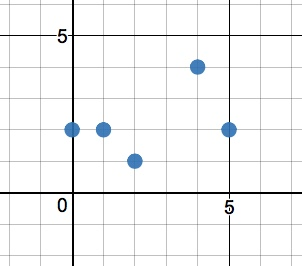
\includegraphics[width=0.35\textwidth]{discrete-domain-graph.jpeg}
    \end{figure}

    \item What is the range of this function modeling a bicycle wheel?
    \begin{figure}[!ht]
        \centering
        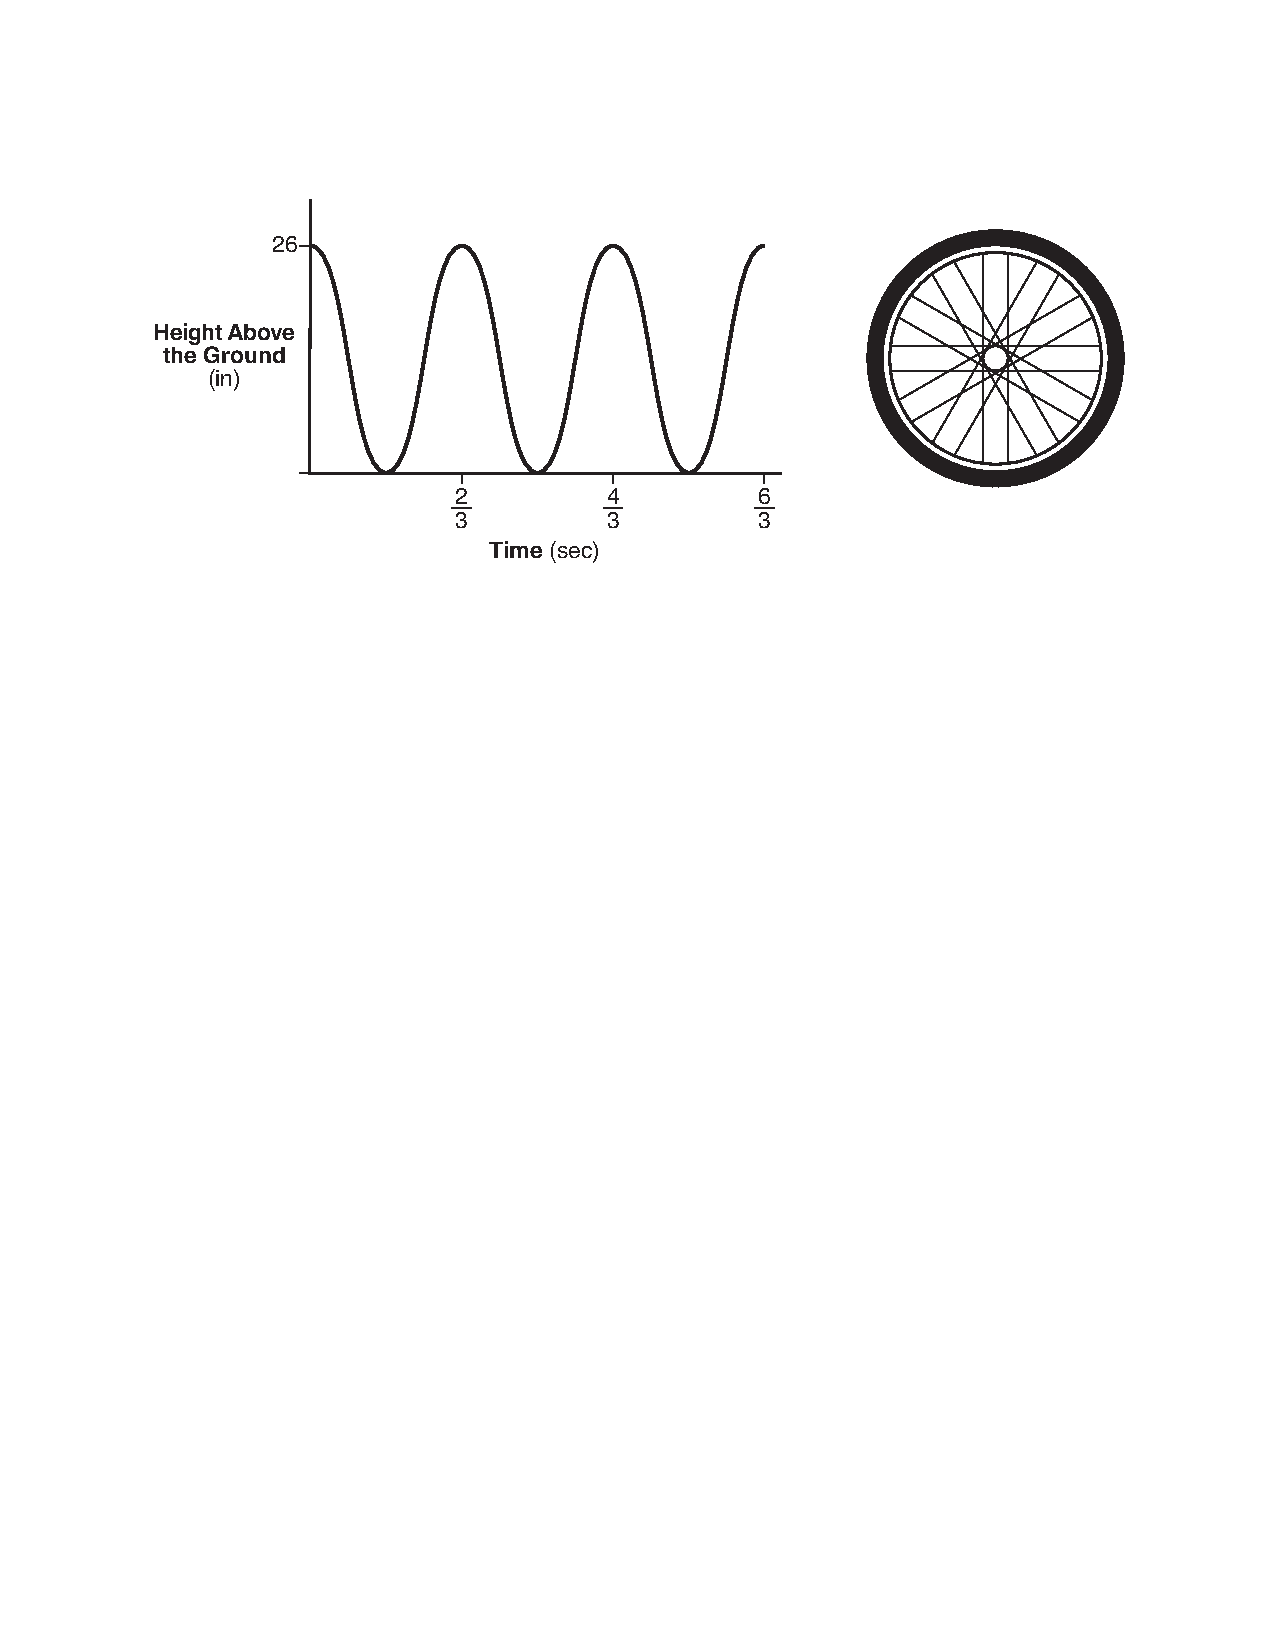
\includegraphics[width=0.70\textwidth]{sine-bike-wheel.pdf}
    \end{figure}
  \end{enumerate}
  }

\frame
{
  \frametitle{Function substitution \hspace{\stretch{1}} \alert{1.5}}
  Given $f(x)=3x+2$. What is $f(2x-1)$? \bigskip
    \begin{enumerate}
        \item Perform the substitution, putting $2x-1$ in parenthesis.\\*[20pt]
        \item Simplify, beginning each line with a leading equals sign if it is equal to the line above.\\*[40pt]
  \end{enumerate}
  }

  \section{1.4 Drui}
  \frame
  {
    \frametitle{GQ: How do we solve quadratic equations?}
    \framesubtitle{CCSS: HSF.IF.B.4 Interpret key features of functions and their graphs \hfill \alert{1.4 Tuesday 10 Sept}}

    \begin{block}{Do Now: Factoring}
    \begin{enumerate}
      \item Find the intercepts, axis of symmetry, and minimum point of the graph of the function $f(x)=(x-1)(x-5)$?
      \item Factor the function $g(x)=x^2-x-12$ to determine the features of its graph.
      \item Convert the function $h(x)=x^2+4x+3$ to the vertex form, $h(x)=a(x-h)^2+k$. Write down its vertex.
    \end{enumerate}
    \end{block}
    Lesson: Factoring, setting $=0$, checking solutions, $x-$ and $y-$intercepts, vertex, axis of symmetry
    \\ \bigskip
    Homework: Factoring practice, completing the square, graphing\\
    Skip around and do what you can by tomorrow
  }

  \section{1.5 Drui - Monday September 17}

  \frame
  {
    \frametitle{How do we graph quadratics?}
    \framesubtitle{CCSS: HSF.IF.B.4 Interpret key features of functions and their graphs \hspace{\stretch{1}} \alert{1.5}}

    \begin{block}{Consider the function $f(x)=-x^2+2x+3$}
    \begin{enumerate}
        \item Factor $f$ and state its zeros.
        \item Restate $f$ in vertex form. Write down the vertex as an ordered pair.
        \item Over what intervals is the function increasing, decreasing, and neither?
        \item If $f(x)$ represents the height of a diver over the domain $0 \leq x \leq 3$, interpret $f(0)$, the vertex, and $f(3)$
        \item What does the "slope" of the curve represent?
    \end{enumerate}
    Lesson: Example 18 p. 54
    \end{block}
  }


\section{1.6 Drui Tuesday September 18th, laptop cart D}
  \frame
  {
    \frametitle{How do we communicate mathematical results?}
    \framesubtitle{CCSS: MP.4 Model with mathematics \hspace{\stretch{1}} \alert{1.6}}

    \begin{block}{Technical skills needed to communicate mathematics}
    \begin{enumerate}
        \item Word processing: Microsoft Word and equation editor
        \item Computer calculators: Desmos; domain restriction, labeling
        \item Cloud storage: Dropbox
        \item Technical writing standards: MLA format (Purdue OWL)
        \item Writing style: declarative
        \item Assessment criteria: IB exploration criterion \emph{B: Mathematics Presentation}
    \end{enumerate}
    \end{block}
    Lesson: Shared folder structure, graph copy/paste, MLA template\\ \bigskip
    Homework: Pre-test
  }

\section{1.7 Drui Review Thursday September 20th}
  \frame
  {
    \frametitle{GQ: How do we simplify exponents?}
    \framesubtitle{CCSS: HSN.RN.A.2 Rewrite expressions involving radicals and rational exponents using the properties of exponents \hspace{\stretch{1}} \alert{1.7}}

    \begin{block}{Do Now: Exponent and radicals practice}
      \begin{enumerate}
      \item Exponent product, quotient, and power rules
      \item Fractional exponents
      \item Negative exponents
      \item Graphing exponential function
      \end{enumerate}
   \end{block}
    Lesson: Product, quotient, power rules, $\sqrt{x^4}$ \\ \bigskip
    Homework: Exponent and radicals practice
  }

\end{document}

\section{1.8 Unit exam September 24th}
  \frame
  {
    \frametitle{GQ: How do we use functions in algebra?}
    \framesubtitle{CCSS: HSF.IF.B.4 Interpret key features of functions and their graphs \hspace{\stretch{1}} \alert{1.8}}

  Exam \\ \bigskip
  Homework: Pre-test
  }
